\documentclass[a4paper,12pt]{article}

%% Language and font encodings
\usepackage[english]{babel}
\usepackage[utf8x]{inputenc}
\usepackage[T1]{fontenc}
\usepackage{ amssymb }
\usepackage{ mathrsfs }
\usepackage{indentfirst}
\setlength{\parindent}{4ex}


%% Sets page size and margins
\usepackage[a4paper,top=3cm,bottom=2cm,left=3cm,right=3cm,marginparwidth=1.75cm]{geometry}

%% Useful packages
\usepackage{amsmath}
\usepackage{graphicx}
\usepackage[colorinlistoftodos]{todonotes}
\usepackage[colorlinks=true, allcolors=blue]{hyperref}
\usepackage{amsthm}

\numberwithin{equation}{section}
\theoremstyle{definition}
\newtheorem{remark}{Axiom}

\title{Cumulative Prospect Theory: A Departure from Expected Utility Theory}
\author{Daniel Banko}

\begin{document}
\maketitle

\section{Introduction}
So far in our consideration of consumer choice theory in class, we have mostly modeled choices devoid of uncertainty. In real-life, however, there is often a likelihood that the scenarios we hope for will not be borne out. For decisions whose outcomes are risky, a common approach in economics is to employ expected utility theory. We will consider an alternative model which brings into question the assumptions underlying expected utility theory.
\subsection{Background}
\indent Kahneman and Tversky's prospect theory, first proposed in 1979 and revised in 1992, is a seminal work in economics. Prospect theory is a descriptive theory that departs from the tradition of assuming economic agents are rational. Kahneman and Tversky, both psychologists, conducted a series of survey experiments to empirically show that rational economic models of utility did not properly reflect people's  choices in the real world. Their 1992 updated version of the theory, known as cumulative prospect theory, retains many of the major features of the original 1979 version, but introduces a (two-part) cumulative function to mathematically represent decision weights when choosing between gambles.

\subsection{Components of Prospect Theory}
The main components of prospect theory are described briefly below and depicted in figure \ref{fig:valuefunction}.
\subsubsection{Gains and Losses from Reference Point}
	Decisions are based on gains and losses from a given reference point. Negative outcomes of prospects are coded as losses and positive outcomes are coded as gains. The reference point is given as the origin on the graph. This point is kinked on the graph.
\subsubsection{Loss Aversion}
	Loss aversion says that losses hurt more than equivalent gains help. That is, it is better to avoid losing $\$5$ than it is to obtain $\$5$. This is represented by the steepness of the value function over losses (left side of graph) relative to equivalent gains (right side of graph).
\subsubsection{Risk-aversion and Risk-seeking Preferences}
	There is diminishing sensitivity to gains and losses such that the value function is concave over gains and convex over losses. This means that people are risk-averse over gains and risk-seeking over losses, i.e. they prefer a gamble to a certainty equivalent over a loss, and the opposite is true for gains.
\\

I now present the 1992 model of prospect theory and its advancements from the 1979 version. Many of the core elements of the original model are retained.

\begin{figure}
\centering
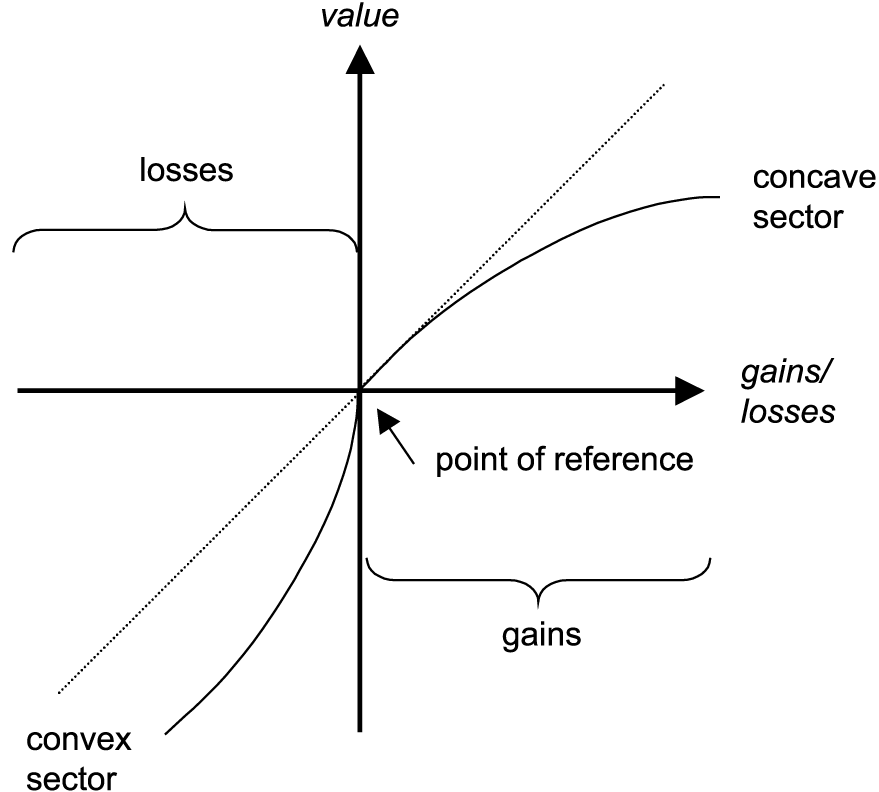
\includegraphics[width=0.7\textwidth]{prospect_theory.png}
\caption{\label{fig:valuefunction} Prospect theory value function.}
\end{figure}

\section{Model}
\subsection{Variables}
\indent  Let $S$ be a finite set of states of nature, where subsets of $S$ are called events. $X$ is a set of outcomes which, for our purposes, will solely be monetary outcomes (Kreps refers to $X$ as prizes). $X$ includes a neutral outcome 0, and we interpret all other elements of $X$ as gains or losses, denoted by positive or negative numbers, respectively.
\\

\indent An uncertain prospect $f$, known as a "gamble," is a function from $S$ into $X$ that assigns to each state $s \in S$ an outcome $f(s) = x$ in $X$. 
\\

\indent To define the cumulative function, we arrange the outcomes of each prospect in increasing order. A prospect $f$ is then represented as a sequence of pairs $(x_i,A_i)$, which yields $x_i$ if $A_i$ occurs, where $x_i > x_j$ iff $i > j$, and $(A_i)$ is a partition of $S$. We will use positive subscripts to denote positive outcomes, negative subscripts to denote negative outcomes, and the zero subscript to denote the neutral outcome.
\\

\indent The positive part of $f$, denoted $f^+$, is obtained by letting $f^+(s) = f(s)$ if $f(s) > 0$, and $f^+(s) = 0$ if $f(s) \leq 0$. The negative part of $f$, denoted $f^-$, is defined conversely.

\subsection{Value and Weight Functions}
\indent We assign to each prospect $f$ a number $V(f)$ such that $f$ is preferred to or indifferent to $g$ iff $V(f) \geq V(g)$. A capacity $W$ is a function that assigns to each $A \subset S$ a number $W(A)$ satisfying $W(\Phi) = 0$, $W(S) = 1$, and $W(A) \geq W(B)$ whenever $A \supset B$ (consider $W$ like a "weight" assigned to a prospect $f$, this will become clear momentarily).
\\

\indent Cumulative prospect theory says that there exists a strictly increasing value function $v:X \rightarrow R$, satisfying $v(x_0) = 0$, with capacities $W^+$ and $W^-$, such that for $f = (x_i, A_i), -m \leq i \leq n$,
\begin{equation}\label{eq:1}
V(f) = \sum_{i=-m}^{n}\pi_iv(x_i)
\end{equation}

and
\begin{eqnarray*}
\pi_n^+ =& W^+(A_n)\\
\pi_{-m}^- =& W^-(A_{-m})\\
\pi_i^+ =& W^+(A_i\cup ... \cup A_n) - W^+(A_{i+1}\cup ... \cup A_n), 0 \leq i \leq n - 1\\
\pi_i^- =& W^-(A_{-m}\cup ... \cup A_i) - W^-(A_{-m}\cup ... \cup A_{i-1}), 1 - m \leq i \leq 0
\end{eqnarray*}

where the decision weight $\pi_i = \pi_i^+$ if $i \geq 0$, and $\pi_i = \pi_i^-$ if $i < 0$. \\

\subsection{Risky Prospects}
The value function above is also defined for risky prospects where $p(A_i)$ is between $0$ and $1$. Instead of $A_i$ as above, we replace it with $p_i = p(A_i)$. In this case, the decision weights are:
\begin{eqnarray*}
\pi_n^+ =& w^+(A_n)\\
\pi_{-m}^- =& w^-(A_{-m})\\
\pi_i^+ =& w^+(p_i+ ... + p_n) - w^+(p_{i+1}+ ... + p_n), 0 \leq i \leq n - 1\\
\pi_i^- =& w^-(p_{-m}+ ... + p_i) - w^-(p_{-m}+ ... + p_{i-1}), 1 - m \leq i \leq 0
\end{eqnarray*}
where $w^+$ and $w^-$ are strictly increasing functions from the unit interval into itself satisfying $w^+(0) = w^-(0) = 0$, and $w^+(1) = w^-(1) = 1$.
\\

In the original prospect theory model, $w^+ = w^-$, which means that gains and losses have equivalent decision weights. The updated model generalizes the original version by allowing for different decision weights for gains and for losses. 
\\

As in the original version, $v$ is assumed to be concave above the reference point ($v''(x) \leq 0, x \geq 0$) and convex below the reference point ($v''(x) \geq 0, x \leq 0$). This is in accordance with the principle of diminishing sensitivity: the impact of a change diminishes with the distance from a given reference point. We also assume that $v$ is steeper for losses than for gains ($v'(x) < v'(-x)$ for $x \geq 0$). This condition is implied by the principle of loss aversion.
\\

In prospect theory, the principle of diminishing sensitivity applies to the weighting functions as well. In the evaluation of uncertainty, there are two endpoints, certainty and impossibility (0 and 1). Diminishing sensitivity entails that the impact of a given change in probability diminishes with its distance from the boundary. It gives rise to a weighting function that is concave near 0 and convex near 1, as demonstrated in figure \ref{fig:weightfunction}. People tend to overweight extreme but unlikely events, but underweight medium to high probabilistic events. Unlike in the original model, it shows different weighting functions for positive and negative prospects.
\\

\indent The 1992 updated version advances the 1979 original model in several respects. First, the cumulative probability function expands the model to infinitely many (i.e. continuous) outcomes. Second, because cumulative probabilities are transformed rather than the probabilities themselves, in the updated version  only prospects with \textit{extreme} payoffs with low probability are overweighted. The original model assumed that people overweighted all unlikely events, independent of their relative outcomes. This led to the original version of prospect theory being susceptible to violations of stochastic dominance: a prospect $f_1$ might be preferred to prospect $f_2$ even if the probability of receiving payoff $x$ in prospect $f_2$ was the same or higher than for prospect $f_1$ for all values of x.



\subsection{Example}
\indent To demonstrate the value function, let's consider an example using a six-sided die. You roll the die once and observe the result $x = 1,...,6$. If $x$ is even, you receive $\$x$; if $x$ is odd, you pay $\$x$. Viewed as a risky prospect, $f$ yields the outcomes (-5,-3,-1,2,4,6) each with probability 1/6. By equation \ref{eq:1}, therefore,
\begin{eqnarray*}
V(f) =& \sum_{i=-m}^{n}\pi_iv(x_i)\\
=& \sum_{i=-m}^{0}\pi_i^-v(x_i) + \sum_{i=0}^{n}\pi_i^+v(x_i)\\
=& v(2)[w^+(1/2) - w^+(1/3)]+v(4)[w^+(1/3) - w^+(1/6)] + v(6)[w^+(1/6)] \\
+& v(-5)[w^-(1/6)]+v(-3)[w^-(1/3) - w^-(1/6)]v(-1)[w^-(1/2) - w^-(1/3)].
\end{eqnarray*}

In the original prospect theory model, $w^+=w^-$. Faced with this gamble (disregarding loss aversion), you would be indifferent between this gamble and a certain outcome of $\$0$, i.e. declining the gamble. In cumulative prospect theory, depending on your decision weights, you could value this gamble net positively or negatively. For example, you may be more risk-averse over gains than you are risk-seeking over losses: this would be demonstrated by $w^+>w^-$. This means you overweight low probabilities of gains more than you overweight low probabilities of losses. Thus, the gamble may be attractive to you if $V(f) > 0$.

\section{Deviations from Expected Utility Theory}

In expected utility theory, the expected value of a set of utilities over possible outcomes $x_i$ is 
\begin{equation*}
{U} = \sum_{i=1}^np_iU(x_i)
\end{equation*} which is linear in the probabilities $(p_i)$.
Probabilities are objective; they are included as part of the description of a choice object. Expectations accurately reflect probabilities and utility is measured as a non-decreasing function of wealth. A prospect is acceptable so long as the final state of wealth is greater. Finally, marginal utility decreases as wealth increases; that is, people are \textit{always} risk-averse.
\\

In prospect theory, probabilities are subjective; empirical evidence suggests that people struggle to weigh probabilities as a continuum. This non-linearity leads to violations of axioms assumed in expected utility theory, such as the independence axiom. This is demonstrated in the Allais Paradox, a version of which is presented below from Kreps.

\begin{figure}
\centering
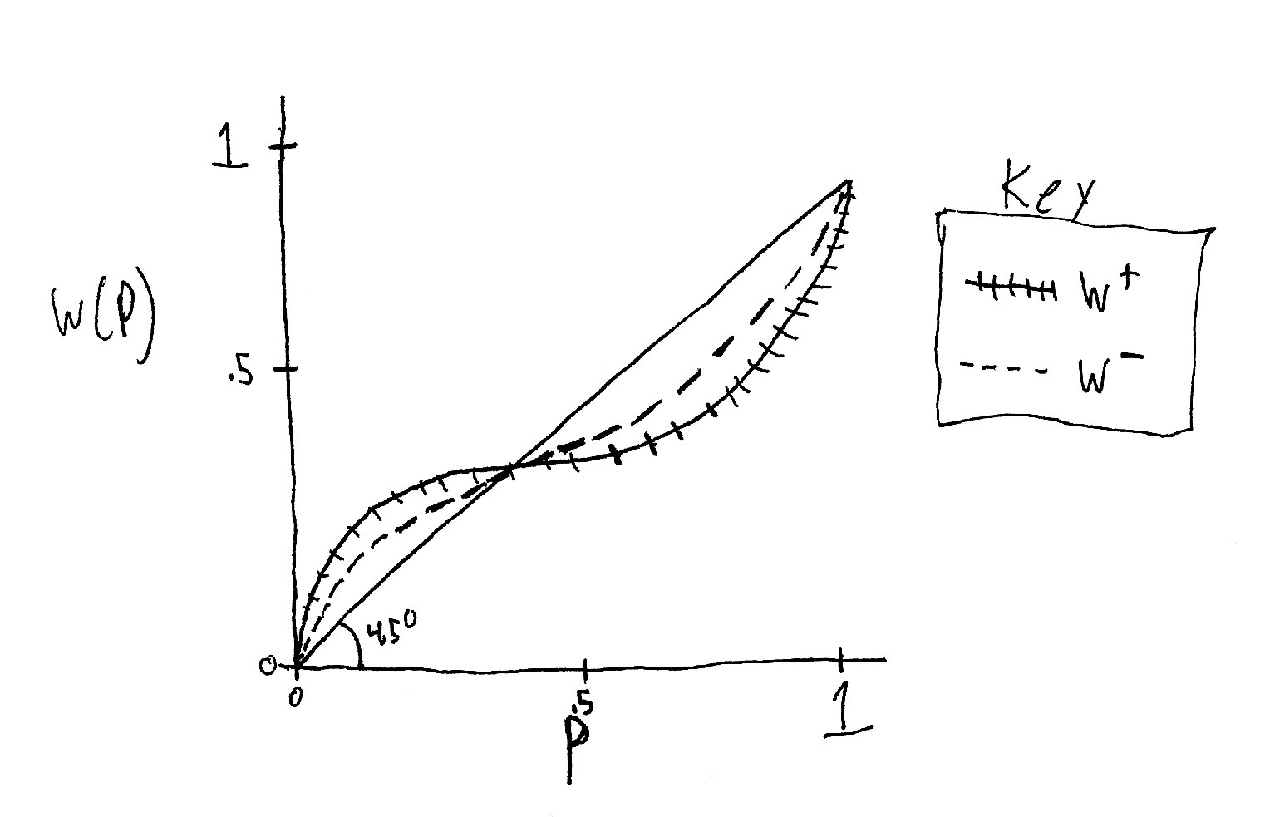
\includegraphics[width=0.7\textwidth]{weightingfunction.pdf}
\caption{\label{fig:weightfunction} Cumulative prospect theory weight function. }
\end{figure}

\subsection{Allais Paradox}
Choose between two gambles. $f$ gives a $.33$ chance of $\$27,500$, a $.66$ chance of $\$24,000$, and a $.01$ chance of nothing. $g$ gives $\$24,000$ for sure.
\\

Now consider a different set of gambles: $f'$ gives a $.33$ chance of $\$27,500$ and a $.67$ of nothing. $g'$ gives a $.34$ chance of $\$24,000$ and a $.66$ chance of nothing.
\\

The typical response is to choose $g$ in the first case, and $f'$ in the second. This response pattern violates the independence axiom: 

\begin{remark}{Independence Axiom.}
If $X \succ Y$, then $P(X) + (1-P)Z \succ P(Y) + (1-P)Z$ for all Z.
\end{remark}

Essentially, the ranking of X and Y does not depend on the choice-maker's preference for Z. Expected utility theory says that adding or subtracting equal outcomes to each choice should have no effect on the relative desirability of one gamble over the other; equal outcomes "cancel" each other out.
\\

How does the Allais Paradox show that this axiom is violated? Choosing $g$ in the first gamble suggests
\begin{equation}\label{eq2}
 24,000 > .33(27,500) + .66(24,000) + .01(0) 
\end{equation}

Choosing $f'$ in the second gamble suggests
\begin{equation}\label{eq3}
.34(24,000) + .66(0) < .33(27,500)+.67(0) 
\end{equation}
\ref{eq2} is equivalent to 
\begin{eqnarray*}
.34(24,000) > .33(27,500)+.01(0)\\
.34(24,000) > .33(27,500)+[.67(0)-.66(0)]\\
.34(24,000) + .66(0) > .33(27,500)+.67(0)\\
\end{eqnarray*}

which violates the preference shown in \ref{eq3}. $f$ and $f'$ have the same relative probabilities of outcomes.
\\

Finally, prospect theory assumes people are risk-seeking over losses, which opposes expected utility's assumption that people are always risk-averse. The utility function is concave over all outcomes in expected utility, whereas it is convex over losses in prospect theory.


\section{Application: Apartment Searching}
Choosing an apartment is a good example of a decision made under uncertainty; one does not know exactly how much a particular apartment is worth because it is hard to gain accurate information about the experience of living in one before agreeing to a lease.
\\

We can model an apartment as a prospect $f$, which has a probability $p(x)$ of an outcome $x$. We assume that prices are not always accurate signals of an apartment's inherent value: apartments can be over or under-priced. $x$ can be defined as the difference (positive or negative) between the sales price and the actual value of the apartment. Furthermore, we assume this difference is immediately attainable in that the individual can take the apartment and sell it to another person in cash at the adjusted price in order to earn/lose the difference in value. This allows us to compare apartments according to their monetary payoff, adjusting for probability. For example, an apartment with a  monetary outcome of $\$5,000$ gives the consumer $\$5,000$ in surplus rent money (the apartment was rented for $\$5,000$ less than it was worth).
\\

We will model two apartments as prospects and analyze the differences between expected utility theory and prospect theory in determining which apartment to choose.
Assume an individual is trying to find an apartment in Washington DC (this person may or may not be the author of this paper). Assume that this individual is quite wealthy and has $\$55,000$ cash in hand. They plan to rent an apartment for one year and pay for it outright, at its posted sale price. They are deciding between two apartments, A or B, that each cost $\$30,000$ to rent for one year. The potential buyer assesses probabilities of the monetary outcomes for both apartments, and will decide to rent the apartment which has the higher expected value.
\\

Apartment A has probability $.5$ of outcome $\$0$ (that is, the apartment is worth exactly the amount that the customer would pay for it), $.25$ of -$\$5,000$ and $.25$ of +$\$5,000$. Apartment B has a higher probability $.9998$ of $\$0$, but a  small chance $.0001$ of $-\$30,000$ (the apartment is near a storehouse of flammable goods and could burn down the day after moving in) and $.0001$ of $+\$50,000$ (this is the likelihood that the Obamas move in next door and become neighborhood friends).
\\

In expected utility theory, outcomes are assessed in terms of final states of wealth. Apartment A has expected utility of 
\begin{eqnarray*}
E(U) =& 55,000 - 30,000 + 
.5(0)+.25(-5,000)+.25(5,000)\\
=& 55,000 - 30,000 + 0 \\
=& 25,000
\end{eqnarray*}
(we assume for simplicity that the individual's utility function for an apartment is simply the expected monetary payoff of the apartment, i.e. U(x) = x).  Apartment B has expected utility of 
\begin{eqnarray*}
E(U) =& 55,000 - 30,000 + .9998(0)+.0001(-30,000)+.0001(50,000)\\
=& 55,000 - 30,000 - 3 + 5\\
=& 25,002
\end{eqnarray*} Apartment B leaves the customer with higher expected monetary payoff and therefore higher utility. Thus expected utility theory would suggest that the potential buyer should choose apartment B.
\\

Suppose the individual evaluates prospects in terms of gains and losses from a given reference point, as in prospect theory. In this case, our buyer does not care that they have $\$55,000$ cash in hand; their reference point is set at their initial endowment, meaning that they are evaluating their choice from $\$0$ on the prospect theory value function graph. Framing apartments as potential gains and losses from the initial endowment, Apartment A has expected value of $.5(0)+.25(-5,000)+.25(5,000) = 0$ and Apartment B has expected value of $.9998(0)+.0001(-30,000)+.0001(50,000) = -3+5 = 2$.
\\

Now suppose our individual is loss averse: losses hurt five-thirds as much as an equivalent gain helps. In order to accurately compare the value of potential gains to potential losses, we scale our negative outcomes accordingly by a factor of 5/3:
\\

Apartment A now has expected value of 
$(.5(0)+.25(-5,000*\times(5/3))+.25(5,000) = (.5(0)+.25(-8,333.34)+.25(5,000) = -833.34$.
\\

Apartment B now has expected value of $(.9998(0)+.0001(-30,000\times(5/3))+.0001(50,000) = (.9998(0)+.0001(-50,000)+.0001(50,000) = 0$.
\\


Apartment B is still preferred to Apartment A. Now let us consider risk-aversion and risk-seeking over gains and losses, respectively. This means that the individual overweights small probabilities of both gains and losses, as in prospect theory. In cumulative prospect theory, the probabilities of mixed prospects (gambles which have both positive and negative outcomes) do not have to add to 1. This is due to the non-linearity of the weighting function. Our individual, it turns out, overweights the likelihoods of the extreme outcomes in the prospect of Apartment B: the likelihood that Obama would be a next-door neighbor and become a best friend is exaggerated to be $0.01$, and the likelihood that the nearby warehouse would catch fire the day after moving in is exaggerated to be $0.03$.
\\

Apartment A's expected value does not change (-833.34) because cumulative prospect theory says that people only overweight unlikely prospects with extreme outcomes, which Apartment A lacks.
\\

Apartment B now has expected value of
$.9998(0)+.03(-30,000\times(5/3))+.01(50,000) = .9998(0)+.03(-50,000)+.01(50,000) = -\$1000$.
\\


Because of the mixed prospects in both apartments and the extreme outcomes in apartment B, prospect theory suggests that this individual would overweight the extreme outcomes in Apartment B relative to Apartment A. Not only that, loss aversion reduces the attractiveness of both apartments, so that if our decision-maker had a third option of not buying either apartment they would decide not to buy because the expected values of both apartments are negative. If the decision-maker was forced to buy one of the two apartments, they would choose Apartment A according to prospect theory, although expected utility theory would predict Apartment B.


\section{Conclusion}
\indent Theories of choice under uncertainty commonly specify objects of choice, a valuation rule, and characteristics of value functions. In expected utility theory, the objects of choice are probability distributions over wealth, the valuation rule is expected utility, and utility is always a concave function of wealth.
\\

Prospect theory proposes instead that the objects of choice are prospects \textit{framed in terms of gains and losses}, the valuation rule is a \textit{two-part cumulative function}, and the value function is \textit{S-shaped} and the weighting functions are \textit{inverse S-shaped}. This has been shown empirically to be a more accurate model for describing behavior in choices involving risky gambles.
\\

\section{References}
\noindent
\hangindent=0.7cm
Tversky, Amos and Daniel Kahneman. "Advances in Prospect Theory: Cumulative Representation of Uncertainty." Journal of Risk and Uncertainty, 5.4 (1992): 297-323.\\

\noindent
\hangindent=0.7cm
Kahneman, Daniel and Amos Tversky. "Prospect Theory: An Analysis of Decision under Risk." Econometrica, 47.2 (1979): 263-292.?\\


\end{document}